
The starting condition for the blast wave simulations was a region of uniform pressure, density an temperature with in the center a circle of higher pressure.
We did simulations for multiple differences in pressure between the low- and highpressure regions to get a better understanding of the non-linear effects in vicinity of shocks.
	
\begin{figure}[H]
	%\hspace{-1cm}
	\centering
	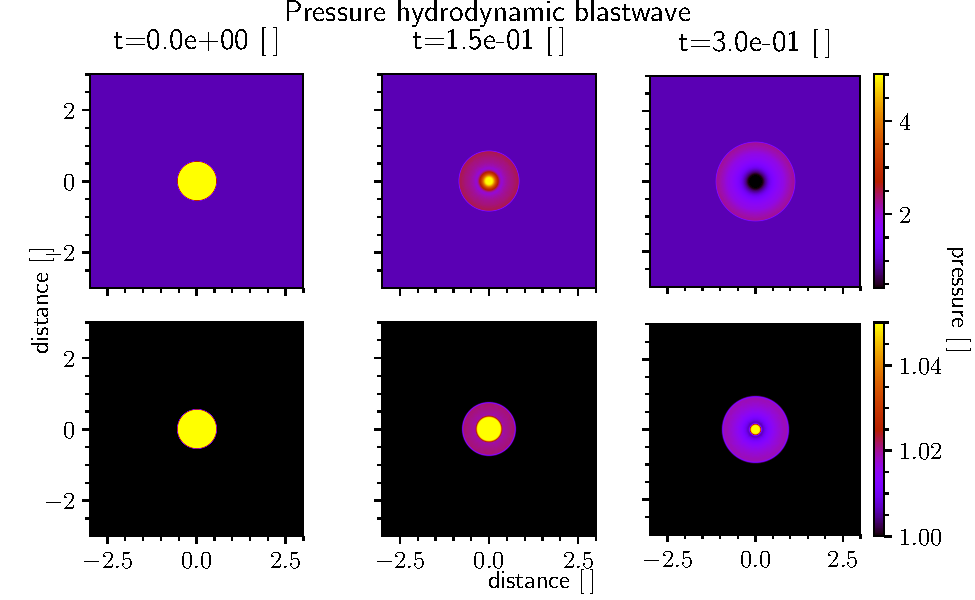
\includegraphics[width=\linewidth]{images/HD-blast-prs-1.pdf}
	\caption{Pressure profile for a blastwave in an ideal fluid at different times. The top row start with the larger pressure difference of $5/1$, the bottom row is the blastwave with smaller pressure difference of $1.5/1$.}
	\label{fig:HD-blast-short}
\end{figure}

\begin{figure}[H]
	%\hspace{-1cm}
	\centering
	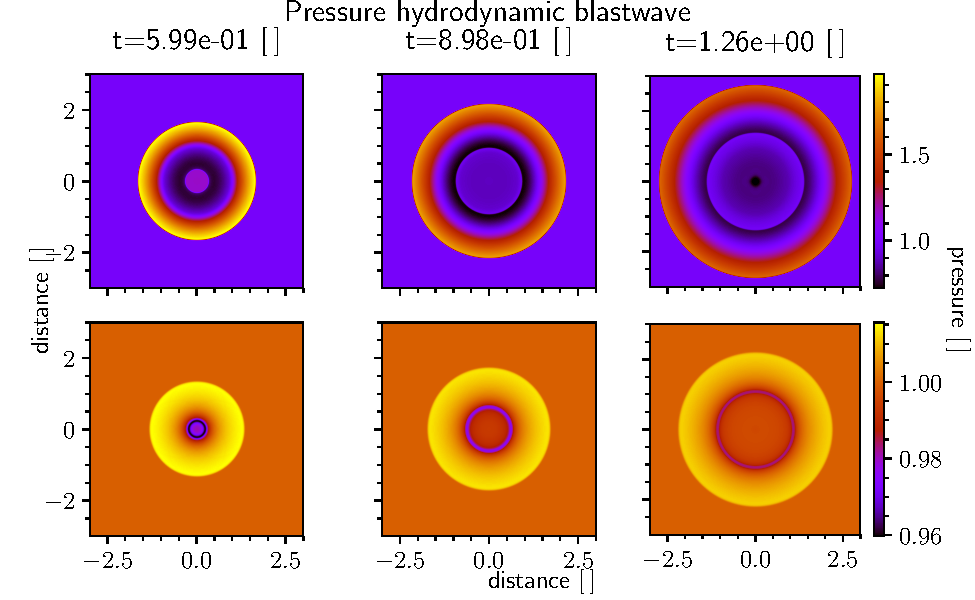
\includegraphics[width=\linewidth]{images/HD-blast-prs-2.pdf}
	\caption{Pressure profile for a blastwave in an ideal fluid at larger timescales. Initial conditions for each row are the same as in \autoref{fig:HD-blast-short}.}
	\label{fig:HD-blast-long}
\end{figure}

